\chapter{Handout 8}

\emph{El documento describe una redada secreta en la \emph{Chapel of
Contemplation}. La operación policial fue impulsada por declaraciones juradas
que acusaban a miembros de la iglesia de estar implicados en la desaparición de
niños del vecindario. Durante la redada, murieron tres policías y diecisiete
miembros de la secta, ya sea por disparos o por el fuego. Los informes forenses
resultan inusualmente vagos y poco detallados, como si el forense no hubiera
llevado a cabo los exámenes adecuados.}

\emph{Aunque fueron arrestados 54 miembros de la iglesia, todos menos ocho
fueron liberados. Los registros sugieren que un alto funcionario local
intervino de manera ilegal en el proceso judicial, y que se relataron versiones
de la redada —la mayor operación criminal en la historia de la ciudad— que
jamás llegaron a publicarse.}

\emph{El pastor Michael Thomas fue detenido y condenado a 40 años de prisión
por cinco cargos de asesinato en segundo grado. Sin embargo, escapó de prisión
en 1917 y huyó del estado.}

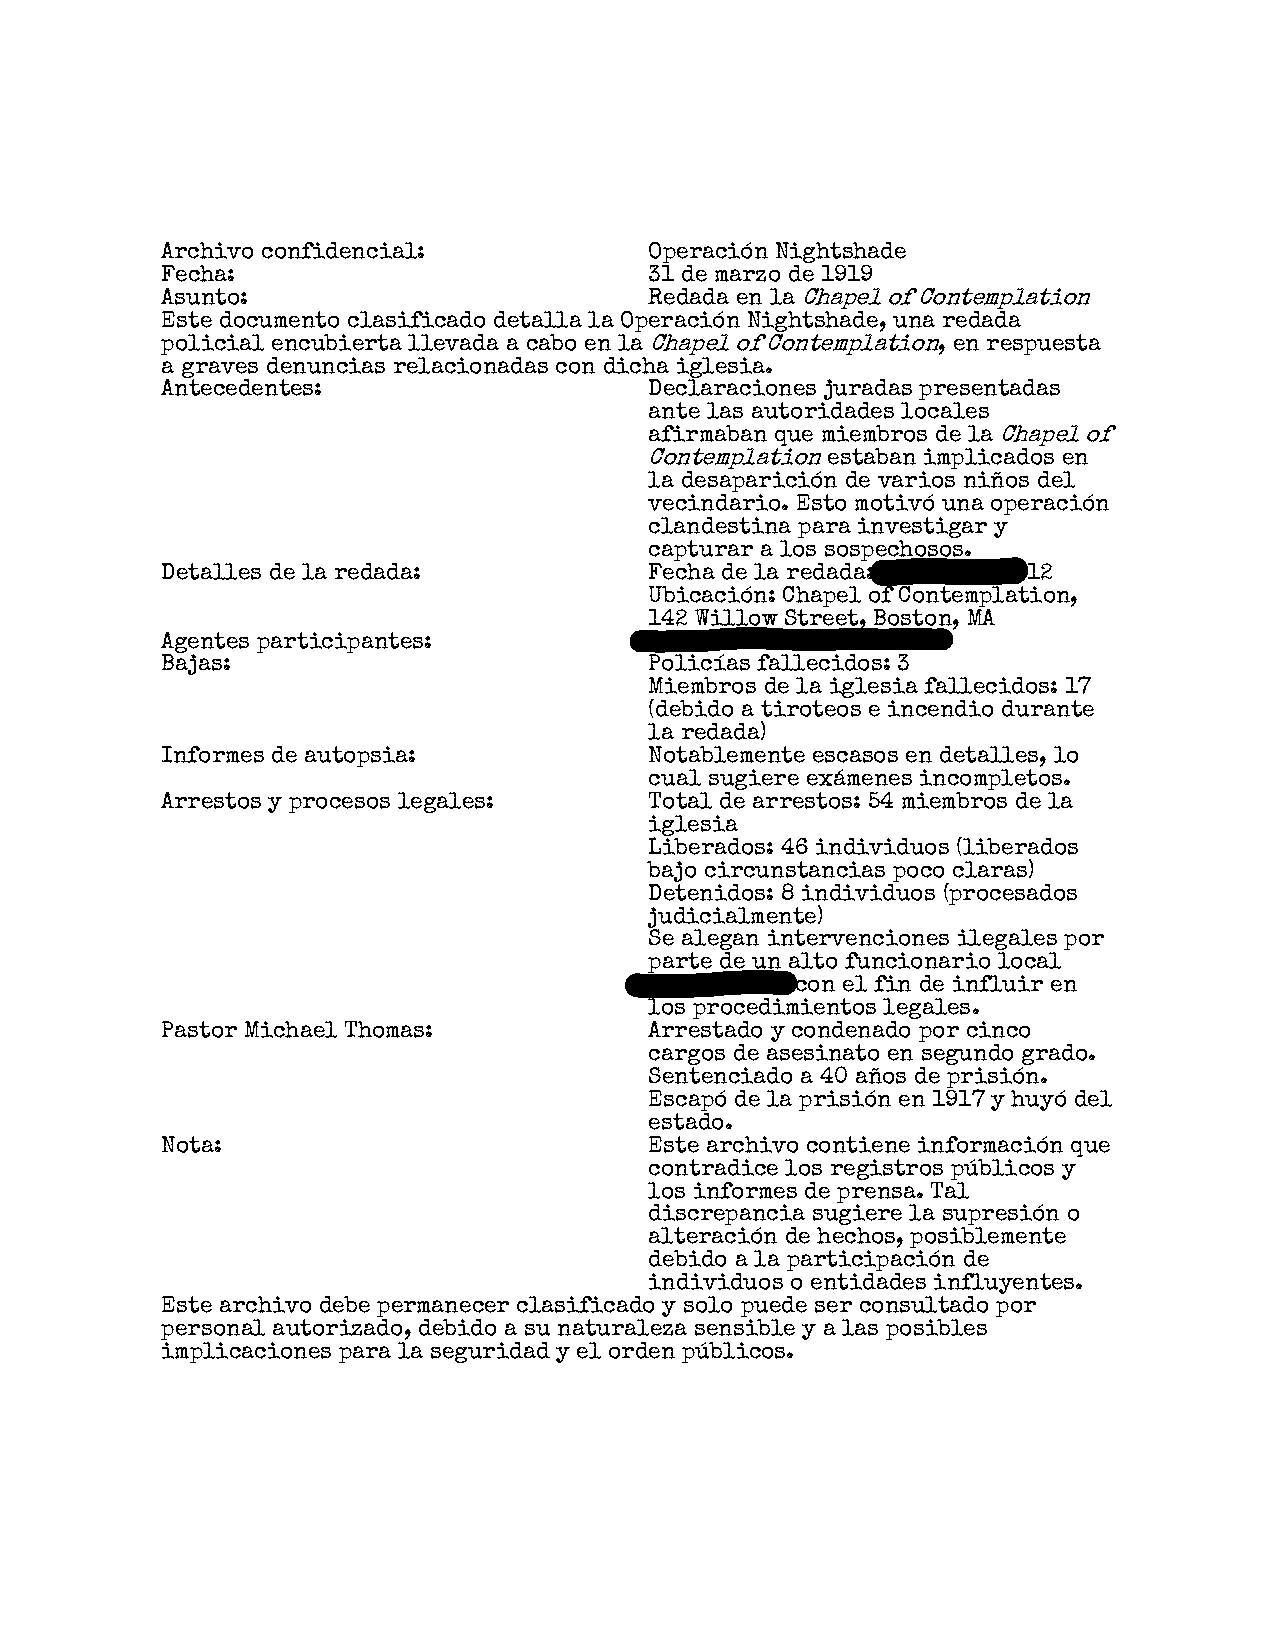
\includepdf[pages={1}, scale=1.0]{./assets/Archivo-confidencial-Operacion-Nightshade.pdf}